\section{Evaluation}
We evaluate our spill-free collision-free trajectory planner, SFRRT*, on the 7DoF Franka Emika Panda robotic arm. We design two scenarios and utilize three different containers with different fill levels (\cref{fig:Training set}, top row) to quantify the performance of SFRRT*. These scenarios are designed to encapsulate real-world use cases of our motion planner, specifically cases that exhibit a diverse range of robot motions: Scenario 1 (\cref{fig:scenario_1_2}, left) involves the robot transporting a drink while avoiding the obstacles on the table; and, Scenario 2 (\cref{fig:scenario_1_2}, right) involves the robot in a chemistry lab transporting a container while avoiding collisions with the fume hood.
Additionally, the containers (wine, flute, and basic glasses) are picked based on their diverse geometries, while the fill levels, ranging from 30\% to 80\% are chosen to cover tasks with varying risks of spillage.
The objective across our evaluation tasks is to move these containers from the start to the goal states without spilling the contents of the container being transported. Each experiment, as enumerated in \cref{table:tasks}, is repeated five times.
\label{sec:experiments-evaluation}
\begin{figure}
\centering
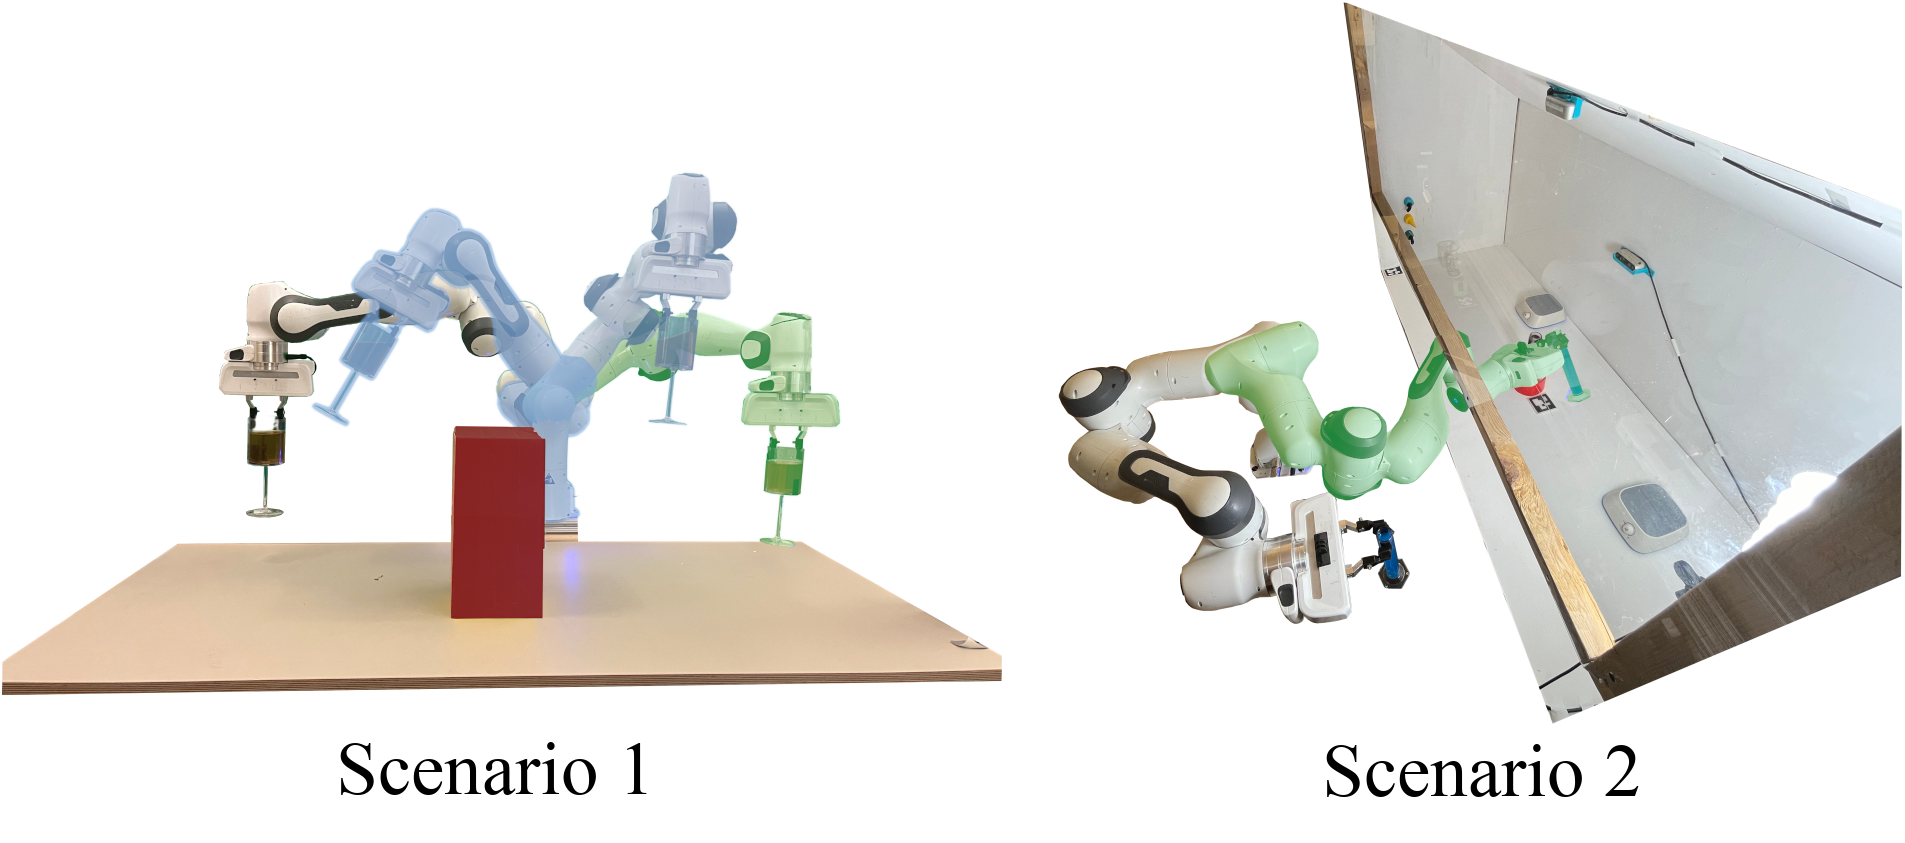
\includegraphics[width=1\columnwidth]{figs/scenario1_2.png}
\caption{
The two scenarios from \cref{table:tasks}: The original colored robot for start position, green for goal. Blue indicates intermediate robot states.
% \vspace{-15pt}
}
\label{fig:scenario_1_2}
% \vspace{-15pt}
\end{figure}
We measure the success rate of SFRRT* (\cref{subsec:successrate}) and compare its obstacle avoidance performance (\cref{subsec:orientation-over-time}) against the SpillNot method from \cite{pendulum}. We also evaluate the accuracy of the SFC model on containers that were not part of the training set, which are also used in the video demo (\cref{scenario 2 gif}) to display a real-world chemistry lab procedure (\cref{sec:eval_no-training-set}). Lastly, we present an ablation study that compares modified versions of the SFRRT* (\cref{sec:eval_ablation}). 
\begin{figure}
    \centering
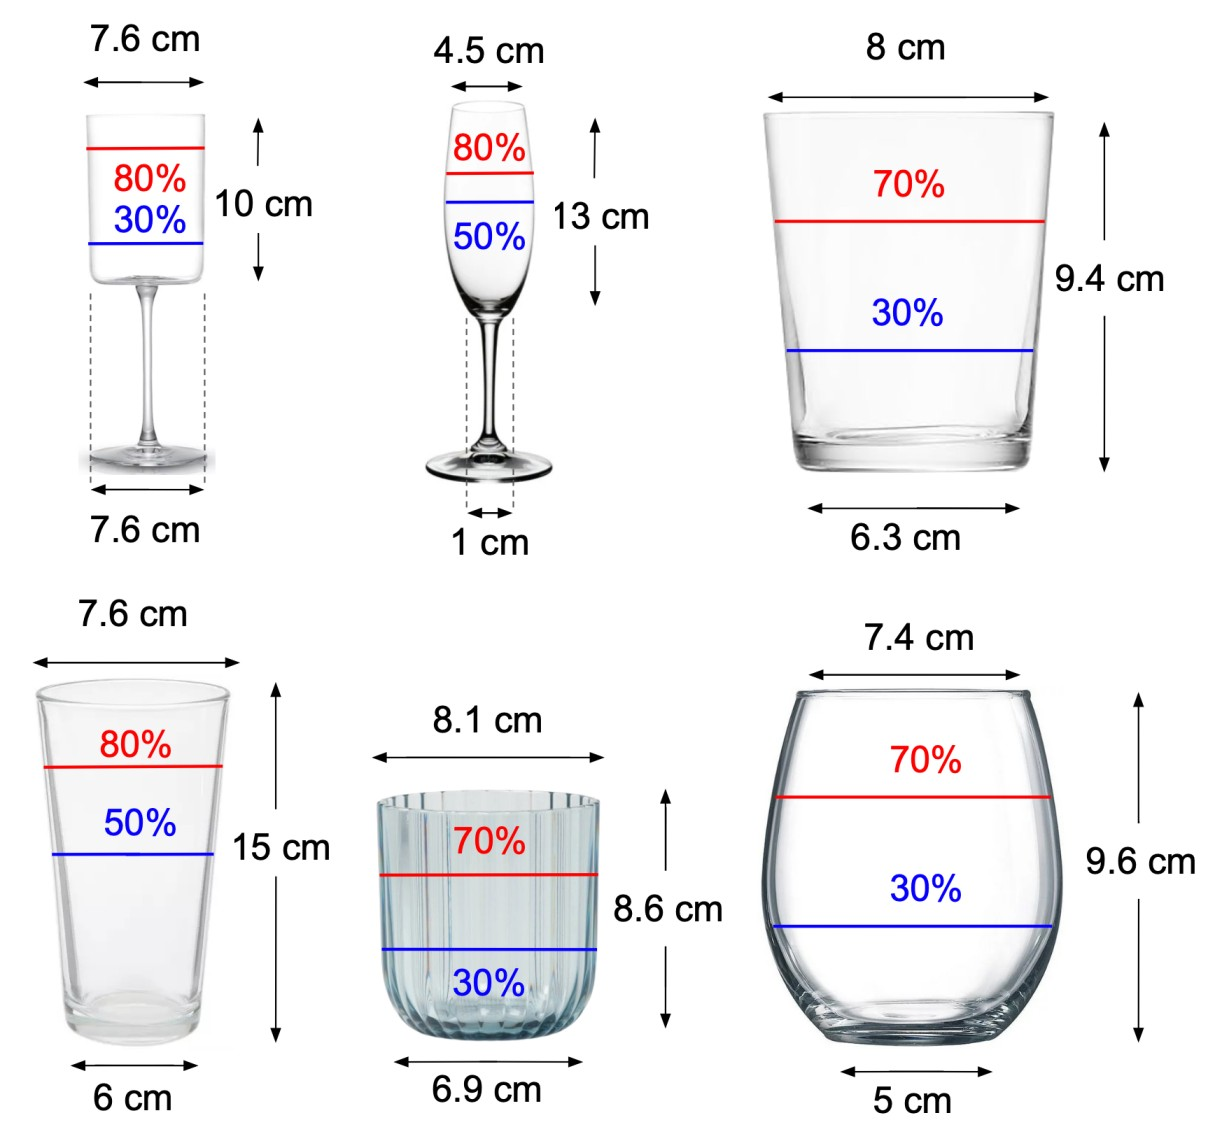
\includegraphics[width=0.7\columnwidth]{figs/training_set.png}
    \caption{The entire set of containers used to train SFC. Notably, the top three containers, identified as the wine glass, flute glass, and basic glass, are used in our experiments.
    }
    \label{fig:Training set}
    % \vspace{-15pt}
\end{figure}
\subsection{Implementation Details}
\label{subsec:implement-details}
The performance of SFRRT* depends on the spill constraint enforced during path planning. This constraint restricts the container's orientation by imposing maximum allowable tilt angles to prevent spillage. As described previously, these angles are calculated using \cref{eq:caseI} and \cref{eq:caseII}. \cref{table:tasks}, last column, presents the maximum tilt angles for the containers used in the experiments. To train the spill-free classifier (SFC) model, we deployed it on TensorFlow and optimized it using a binary cross-entropy loss function for 400 epochs with a batch size of 32. SFC achieved an accuracy of 94\%. Detailed training parameters are available on the open-source code.
\begin{table}[H]
\begin{center}
\begin{tabular}{||c | c | c | c | c||} 
 \hline
Experiment & Scenario & Container & Fill Level & $\theta_{max}$\\[0.5ex] 
 \hline
1 & 1 & Wine glass & 80\% & 39$^\circ$\\
\hline
2 & 1 & Wine glass & 30\% & 65$^\circ$\\
\hline
3 & 1 & Flute glass & 80\% & 49$^\circ$\\ 
\hline
4 & 1 & Flute glass & 50\% & 72$^\circ$\\ 
\hline
5 & 2 & Basic glass & 70\% & 35$^\circ$\\
\hline
6 & 2 & Basic glass & 30\% & 62$^\circ$\\
    \hline
\end{tabular}

\caption{\label{table:tasks} \textbf{Experiments designed for assessing SFRRT*}: Each is repeated 5 times using a Panda robotic arm.
% \vspace{-15pt}
}
\end{center}
\end{table}


% \begin{enumerate}
% \item Scenario 1 - Container 1 - 80\%  
% \item Scenario 1 - Container 1 - 30\%
% \item Scenario 1 - Container 2 - 80\%
% \item Scenario 1 - Container 2 - 50\%
% \item Scenario 2 - Container 3 - 70\%
% \item Scenario 2 - Container 3 - 30\%
% \end{enumerate}
\vspace{-15pt}
Finally, several key parameters are set in SFTP (\cref{alg:sftp}). The bounds on velocity, acceleration, jerk and are set according to the robotic arm's kinematic constraints \cite{panda}. Moreover, the jerk decrease factor $rate$ is set to 2, meaning when SFTP fails to find a spill-free trajectory, $J_{max}$ will be halved and SFTP will reevaluate for spillage under the updated constraint. This $rate$ selection balances execution time and planning time: a smaller rate would extend the time to find a spill-free trajectory, while a larger rate could lead to unnecessarily slow trajectories due to large jerk constraints. 
\subsection{Success Rate}
\label{subsec:successrate} To measure the success rate of the experiments presented in \cref{table:tasks}, each experiment was repeated five times and the result is presented in \cref{table:spill}. Success is defined as the absence of spillage and environmental collisions during the executed motion. Overall, we achieved a 100\% success rate for all experiments except experiment 5.
For experiment 5, spill-free trajectories were accomplished in four out of five trials. Experiment 5 faced challenges since 
it used a container with a maximum tilt angle of 35$^\circ$, smaller than others, limiting the trajectory planning options and increasing spillage risk. Additionally, the SFC model, with its 94\% accuracy, had difficulty adapting to this constrained scenario, contributing to the lower success rate.
\begin{table}[H]
\begin{center}
\renewcommand{\arraystretch}{1.5}
\begin{tabular}{|c | c | c | c | c | c | c |} 
 \hline
Experiment & 1 &  2 & 3 & 4 & 5 & 6 \\[0.5ex] 
 \hline
Success & $5 / 5$ & $5 / 5$ & $5 / 5$ & $5 / 5$ & $4 / 5$ & $5 / 5$ \\ 
 \hline
\end{tabular}

\caption{\label{table:spill} Success rates for different experiments.}
% \vspace{-15pt}
\end{center}
\end{table}



\subsection{Avoiding Obstacles} 
\label{subsec:orientation-over-time}
\begin{figure}
    \centering
    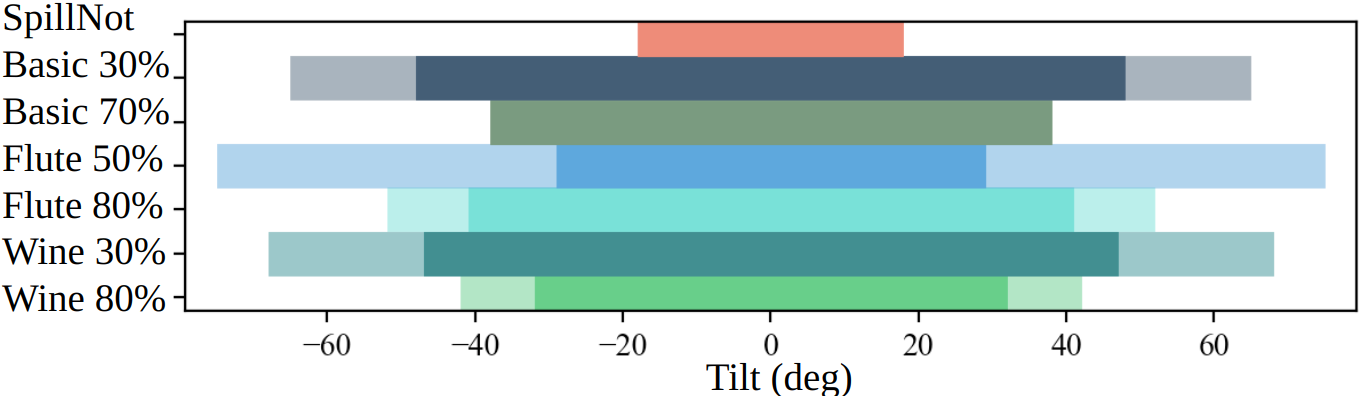
\includegraphics[width=1\columnwidth]{figs/tilt_angle_ranges.png}
    \caption{Maximum tilt angles executed by the robot across all 30 trials from \cref{table:tasks}. 
    The Y Axis labels correspond to the experiments, for example, "Basic 30\%" represents experiment 6. The shaded region represents the allowable maximum tilt angle (\cref{table:tasks}, last column). The solid-colored line corresponds to the executed maximum tilt angle. SpillNot's \cite{pendulum} maximum tilt angle is included for comparison.
    % \vspace{-15pt}
    }
    \label{fig:tilt_angle_for_diff_tasks}
\end{figure}
A key capability of SFRRT* is its ability to navigate around obstacles in the environment while ensuring the container does not spill. To analyze this ability, we focus on the end effector orientation allowable ranges. In SFRRT*, the container orientation is constrained by the maximum tilt angle of the container, i.e. it can generate spill-free trajectories, so long as the container is not tilted past the maximum tilt angle.
By enabling the robot to tilt the container to higher angles, it can more flexibly maneuver in cluttered spaces, such as a fume hood, which may require tilting chemistry vessels to fit them inside.


 To illustrate this expanded ability, \cref{fig:tilt_angle_for_diff_tasks} shows the maximum possible and maximum utilized tilt angles of all 30 trials of \cref{table:tasks}. 
 In every experiment, SFRRT* utilizes a larger tilt range than the SpillNot \cite{pendulum}.
 Notably, SpillNot's tilt angles are not contingent on the fill level and are always limited to a maximum of 15$^\circ$ to maintain low linearization error (\cite{pendulum}, Fig 4).
 We also chose \cite{pendulum} for comparison because, unlike other methods, it does not rely on sensor-based slosh modeling, and allows translational motion in all axes.


As seen in \cref{fig:tilt_angle_for_diff_tasks}, using SFRRT* the robot achieves a maximum tilt angle of 45$^\circ$ when transporting the basic container with a 30\% fill level (\cref{table:tasks}, experiment 6), surpassing the SpillNot method's 15$^\circ$. The range of orientation for this specific container is 3x larger than \cite{pendulum}. Crucially, the maximum tilt angle for the flute glass with a 70\% fill level is 72$^\circ$, a 4.8x increase in orientation range.


Furthermore, it is important to enable orientation changes along all axes to avoid obstacles. For example, maintaining a fixed pitch angle throughout the trajectory prevents avoidance of obstacles in certain cluttered environments. SFRRT* can generate trajectories where all three axes of orientation are utilized. \cref{fig:all_trajectories} displays the container orientation over all the 30 trajectories generated for \cref{table:tasks}. As shown, there are changes in Euler angles across all axes, the range for roll, pitch, and yaw angles are $[-49, 41]$, $[-30, 30]$, and $[-16, 9]$ degrees, respectively. In contrast, the SpillNot method imposes a fixed yaw angle throughout the trajectory \cite{pendulum}. 
% \input{tables/euler_angles}

\begin{figure}
    \centering
    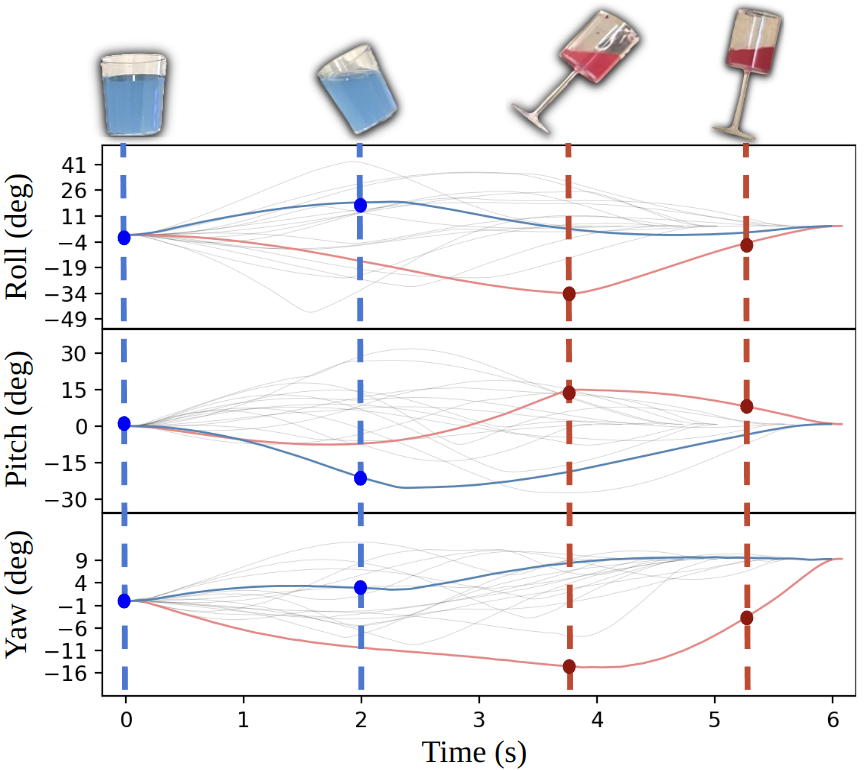
\includegraphics[width=1\columnwidth]{figs/roll_pitch_yaw_final.png}
    \caption{Container orientation over time across all 30 trials from \cref{table:tasks}. The red and blue lines are two trajectories generated for experiment 1 and experiment 6 respectively. Snapshots of the container at specific Euler angles are displayed at the top of the plot. As seen, there are angle changes in each axis of orientation, highlighting the ability of SFRRT* to avoid obstacles.}
    \label{fig:all_trajectories}
\end{figure}

\subsection{SFC: Generalization Capability and Velocity Adaptation}\label{sec:eval_no-training-set}
\begin{figure}
\centering
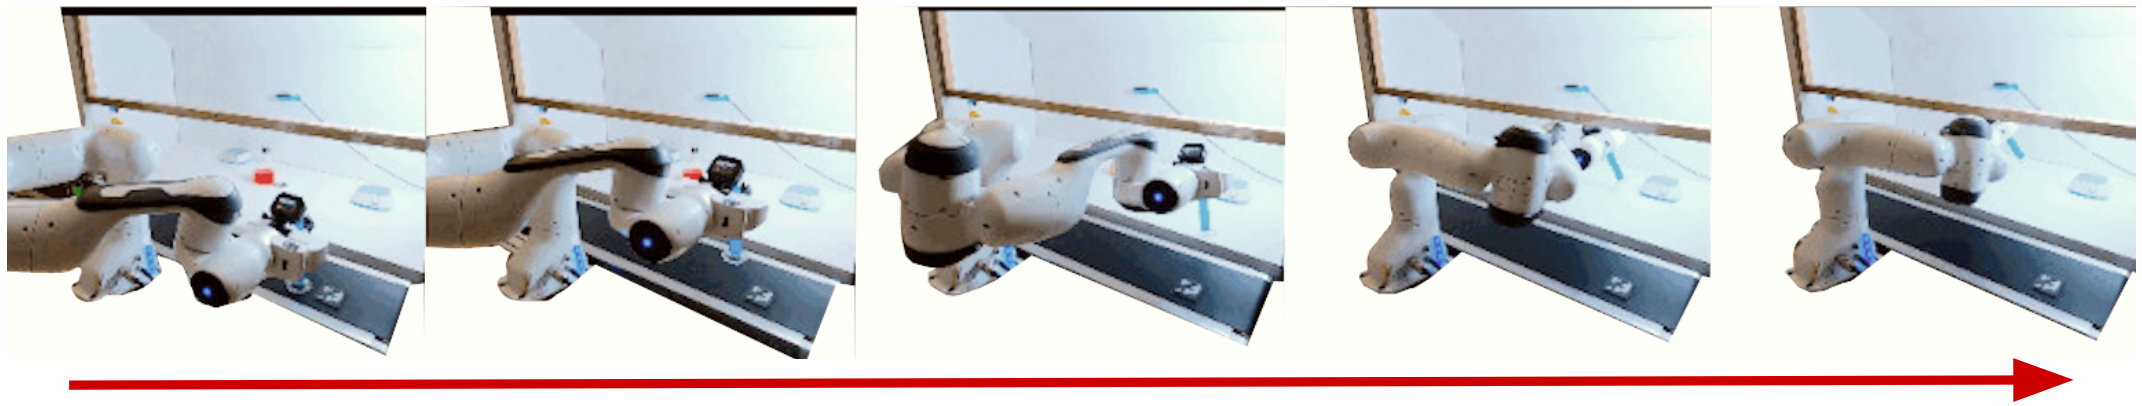
\includegraphics[width=1\columnwidth]{figs/scenario2_vid.png}
\caption{The robot transporting a graduated cylinder into the fume hood while avoiding spills and collisions}
\label{scenario 2 gif}
% \vspace{-15pt}
\end{figure}
The Spill-Free Classifier (SFC) model is trained using 75\% of the 700 trajectories and achieved an accuracy of 94\% for the validation set.
To evaluate the generalization capability of the SFC, its accuracy was tested on novel containers not present in the training dataset. Specifically, a round bottom flask, beaker, and graduated cylinder were used to gather multiple trajectories using a motion capture system (\cref{table:gene}). For each container type, 12 trajectories were gathered with varying fill levels.


As shown in \cref{table:gene}, SFC demonstrates good generalization capability. It achieves strong performance for the beaker and graduated cylinder, with 11 out of 12 data points accurately predicted. However, its accuracy is lower for the round bottom flask, with only 8 out of 12 data points predicted correctly. This is because the SFC model input for container properties only includes details that capture curvy-shaped containers by estimating them to a frustum of a cone. By representing these shapes as frustums of cones, the SFC model ensures a conservative yet safe portrayal of container properties. While this cautious approach may occasionally lead to conservative false negatives, it guarantees the generation of spill-free trajectories.

We also explore a different model architecture for SFC. The current architecture (\cref{fig:models}) passes only the trajectory to the transformer layer before concatenating with container properties. We modified this by concatenating properties at each trajectory step before passing it to the transformer. We call this modified architecture SFC$_m$. SFC$_m$ achieved only 88\% accuracy, lower than the 94\% of SFC, and demonstrated lower accuracy on novel containers than SFC (\cref{table:gene}).
\begin{table}[H]
\begin{center}
% \setlength{\abovecaptionskip}{0pt}
% \setlength{\belowcaptionskip}{0pt}
% \vspace{-14pt}
\renewcommand{\arraystretch}{1.5}
\begin{tabular}{|c | c | c | c|} 
 \hline
 &
    \begin{minipage}{.2\columnwidth}
        \begin{center}
          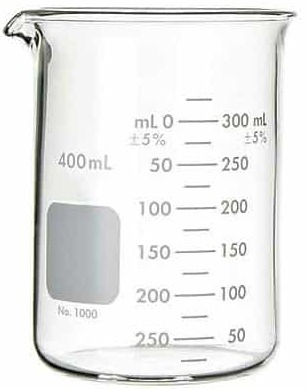
\includegraphics[width=.5\columnwidth]{figs/beaker.png}
        Beaker
        \end{center}
    \end{minipage}
 & 
     \begin{minipage}{.2\columnwidth}
     \begin{center}
      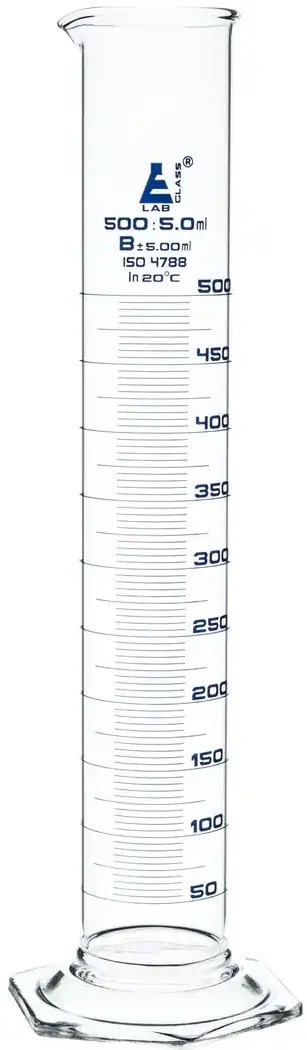
\includegraphics[width=.23\columnwidth]{figs/cylider.png}

      
      Graduated Cylinder
    \end{center}
    \end{minipage}
& 
    \begin{minipage}{.2\columnwidth}
    \begin{center}
      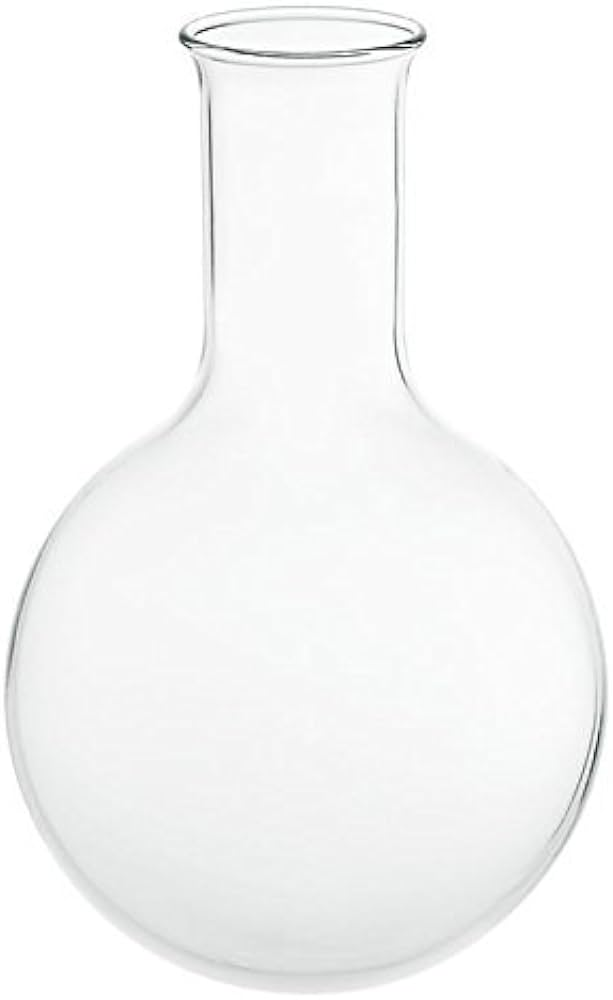
\includegraphics[width=.5\columnwidth]{figs/round_bottom_flask.png}

      
      Round Bottom Flask
    \end{center}
    \end{minipage}
 \\\hline
\textbf{SFC} & \textbf{$11 / 12$} & \textbf{$11 / 12$} & \textbf{$8 / 12$} \\\hline
SFC$_{m}$& $8 / 12$ & $9 / 12$ & $8 / 12$ \\\hline
\end{tabular}
\caption{\label{table:gene} Model accuracy using unseen containers. SFC demonstrates robust performance in predicting outcomes with previously unseen containers, outperforming SFC$_m$.
}
% \vspace{-12pt}
\end{center}
\end{table}

Lastly, SFC is able to take advantage of the container shape to generate trajectories with different velocities. As seen in \cref{fig:mean-vel}, considering the same containers, with different fill levels we see that it consistently generates higher velocities for containers with lower fill levels, which are less likely to spill. Moreover, when comparing different containers in the same scenario (as in \cref{table:tasks}), those with higher tilt angles consistently achieve higher velocities. For example, in the comparison between the wine glass and the flute glass, the wine glass consistently achieves lower mean velocities. This is attributed to the geometry of the containers. As shown in \cref{table:tasks}, the wine glass has a lower maximum tilt angle compared to the flute glass, indicating smaller room to maneuver and a higher susceptibility to spillage. Conversely, the flute glass, with its higher maximum tilt angle consistently achieves higher mean velocities.
\subsection{Ablation Study}\label{sec:eval_ablation}
In this section, two key elements of SFRRT* are modified to evaluate their impact on performance: the informed sampler and the spill-free classifier (SFC) model.
\begin{table}[H]
\begin{center}
\renewcommand{\arraystretch}{1.5}
\begin{tabular}{|c | c | c| c|} 
 \hline
 Task & \textbf{SFRRT*} & SFRRT*$_{u}$ & SFRRT*$_{r}$ \\\hline
  1 & \textbf{$5 / 5$} & $0 / 5$ & $1 / 5$ \\\hline 
  2 & \textbf{$5 / 5$} & $1 / 5$ & $1 / 5$ \\\hline
\end{tabular}

\caption{\label{table:ablation} \textbf{Success Rate Comparison:} 
SFRRT*$_{u}$ uses a uniform sampler, while SFRRT*$_{r}$ skips the SFC spillage checks and uses random sampling for jerk constraints in time parameterization. Overall, SFRRT* outperforms all variants.
% SFRRT*$_{u}$ utilizes a uniform sampler, while SFRRT*$_{r}$ excludes the SFC model for spillage checks, instead opting for random sampling of jerk constraints for time parameterization. As depicted, SFRRT* outperforms all variations significantly.
}
\end{center}
\end{table}

\textit{Informed Sampler Variation: SFRRT*$_{u}$.}
To avoid sampling states such as an upside-down container, or a container tilted beyond its capacity, the informed sampler samples states within the maximum allowable tilt angles for the container (\cref{table:tasks}, last column). To measure its impact, we replace it with a uniform sampler, creating SFRRT*$_{u}$. Then, experiments 1 and 2 are executed 5 times on the robot, and the success rate is shown in \cref{table:ablation}. The success rate drops significantly since the path generation lacks state sampling constraints, as a result, the time parameterization algorithm struggles to create a spill-free trajectory using this path.


\textit{Spill-Free Classifier Variation: SFRRT*$_{r}$.}
In SFRRT*, the SFC model assists with time parameterization by selecting the jerk constraints to ensure a spill-free trajectory. To evaluate the impact of SFC, we introduce SFRRT*$_{r}$ by replacing the SFC model with a random jerk selection. More specifically, a random jerk is selected out of all the jerks that were ever chosen by SFC. The path is then parameterized using that jerk. \cref{table:ablation} shows the success rate for experiments 1 and 2. The observed drop in success rate is due to the random selection of jerk constraints without considering the path itself, in contrast to using the SFC model which takes the path into account when choosing the jerk constraints.

\begin{figure}
    \centering
    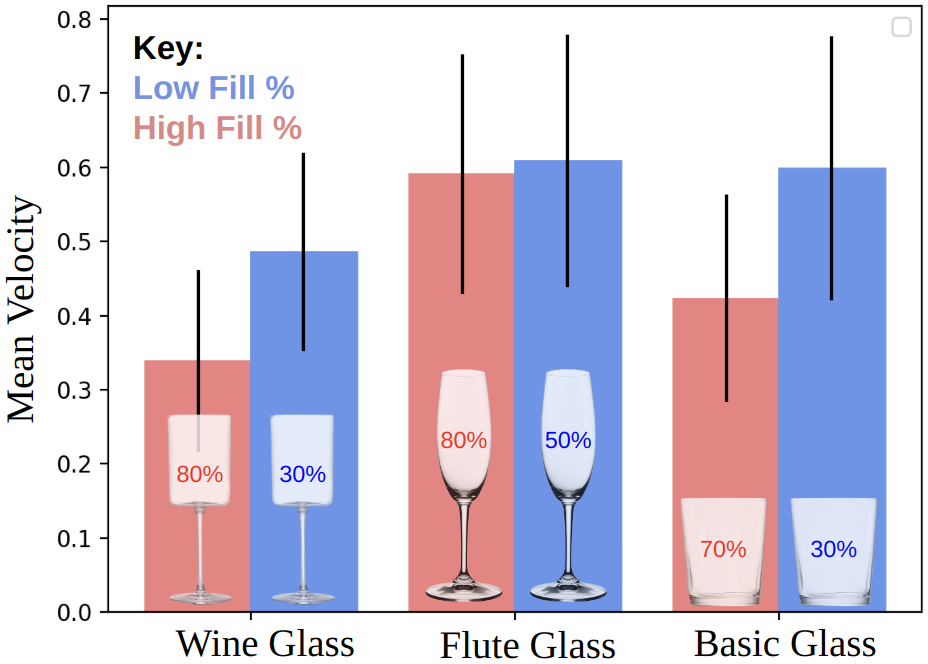
\includegraphics[width=0.8\columnwidth]{figs/mean_vel_fff.png}
    \caption{\textbf{Executed Mean Velocity for Containers from \cref{table:tasks} Using SFRRT*} As depicted, SFRRT* performs faster trajectories for containers with lower liquid fill levels.
    % \vspace{-15pt}
    }
    \label{fig:mean-vel}
\end{figure}


% This is limiting, because cases where the robot has to tilt a container to avoid an obstacle are limited whereas in our approach the container can be tilted as high as the maximum tilt angle.  This inherent limitation poses challenges in scenarios with obstacles, as the planner in \cite{pendulum} struggles to find a spill-free solution when the container needs to tilt beyond $15^\circ$.

% The trajectory generated for experiment 3, illustrated in \cref{fig:task_3_trajectory}, exemplifies the adaptability of our algorithm. Throughout the experiment, noticeable changes in orientation occur across all axes.
% \cref{fig:task_3_trajectory} displays a trajectory generated for experiment 3. As shown, there are angle changes in all of the axes. Moreover, \cref{table:euler_angles} presents the ranges of the end effector Euler angles that were executed across all tasks. As we see there are significant changes in each axis.  In comparison, in \cite{pendulum} the yaw angle is constant. 
% Moreover, the maximum tilt angles executed by the robot for all the experiments are presented in \cref{fig:tilt_angle_for_diff_tasks}. As shown, the highest tilt angle executed by the robot is 45$^\circ$ in task 6. This is while the SpillNot method \cite{pendulum}, has a max tilt angle of 15$^\circ$.

% To evaluate the capability of SFRRT*, in avoiding obstacles while maintaining a spill-free trajectory, we examine the constraints we impose on the robot.


% Given the sampling-based nature of our approach, the informed sampler is designed to sample any state within the robot kinematic constraints, as long as the orientation of that state falls within the maximum tilt angle as outlined in \cref{table:max_tilt_angle}. This implies that the robot can effectively generate a spill-free trajectory for a given container, provided that the container orientation does not exceed the maximum tilt of the container. Consequently, in scenarios where the container's tilt remains within the specified maximum angle, the robot can successfully generate a spill-free trajectory. \ava{mention yaw}

% For instance, the green line in \cref{fig:euler_angles} shows the orientation of the container for a trajectory generated for task 6 (\cref{table:tasks}). Notably, we see that the trajectory has a significant angle change in each of the three axes of rotation. Additionally, the container is tilted as high as 40$^\circ$. In contrast, the red line in \cref{fig:euler_angles} shows the tilt angle variation over time for the SpillNot method presented in \cite{pendulum}. 
% The method outlined in \cite{pendulum} employs a linearized spherical pendulum model, resulting in a constrained tilt angle of less than 15$^\circ$. 

% This inherent limitation poses challenges in scenarios with obstacles, as the planner in \cite{pendulum} struggles to find a spill-free solution when the container needs to tilt beyond $15^\circ$. 


% \subsection{Velocity Over Time}
% In this section, we examine how the SFC model has adjusted the trajectory velocity for different containers with different fill levels (\cref{alg:sftp}). In \cref{fig:mean-vel}, we present the mean and standard deviation of velocities across the 6 tasks mentioned in \cref{table:tasks}. The mean velocity, derived from the average of five trials for each task, demonstrates the model's proficiency in adapting to containers with varying fill levels. Notably, the model consistently generates higher velocities for containers with lower fill levels, indicative of their increased stability and reduced susceptibility to spillage.

% For a more detailed comparison, consider the wine glass and the flute glass, which are subjected to the same scenarios (tasks 1, 2, 3, and 4). The mean velocity for the wine glass consistently surpasses that of the flute glass. This disparity in velocity is attributed to the inherent geometry of the containers. As seen in \cref{table:max_tilt_angle}, the wine glass has a consistently lower max tilt angle than the flute glass, meaning the wine glass is more prone to spillage. In contrast, the flute glass, with its higher maximum tilt angle and thus a safer spill-free design, exhibits higher mean velocities across tasks.